\section{Event Observable Distributions}

In this section, several kinematic distributions from jets and muons 
are shown for each MC sample.


\subsection{Jet Kinematics}
\begin{figure}[htbp]
  \begin{center}
    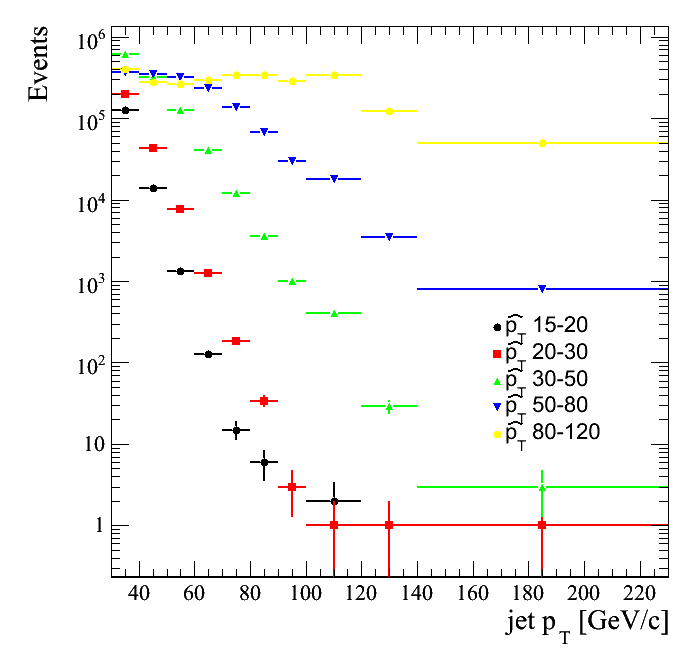
\includegraphics[width=80mm]{Figures/jet_ptqcdbinned.png}
    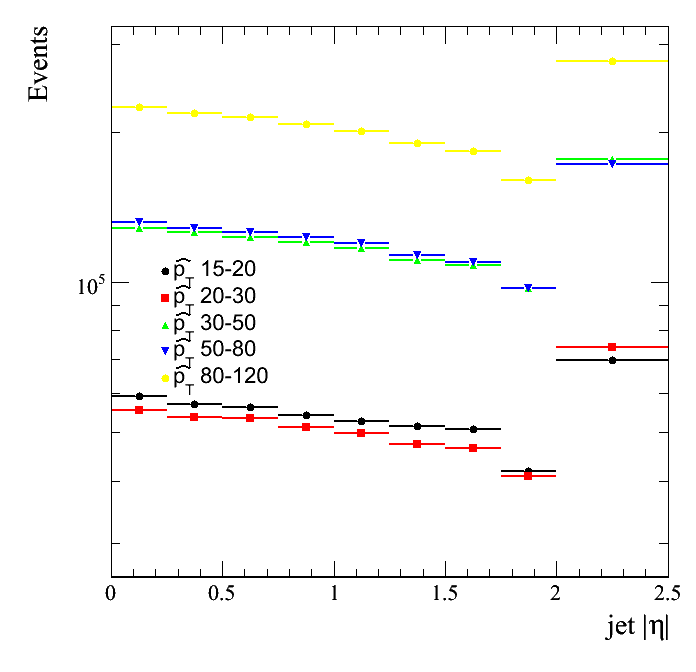
\includegraphics[width=80mm]{Figures/jet_eta_qcdbinned.png}
  \end{center}
  \caption{Jet $p_T$ and $eta$ distributions from the QCD samples $15<\hat{p_T}<120$~GeV/c.}
  \label{fig:jet_pt_QCD}
\end{figure}

\begin{figure}[htbp]
  \begin{center}
    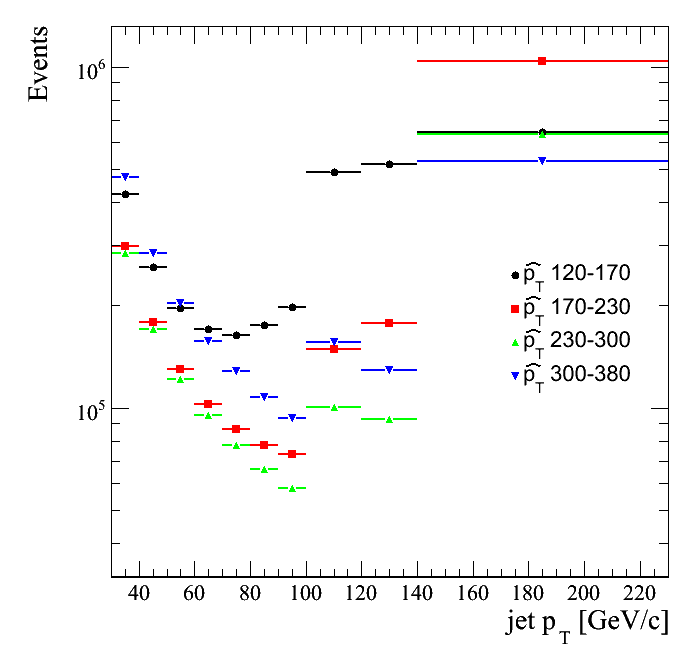
\includegraphics[width=80mm]{Figures/jet_pt2qcdbinned.png}
    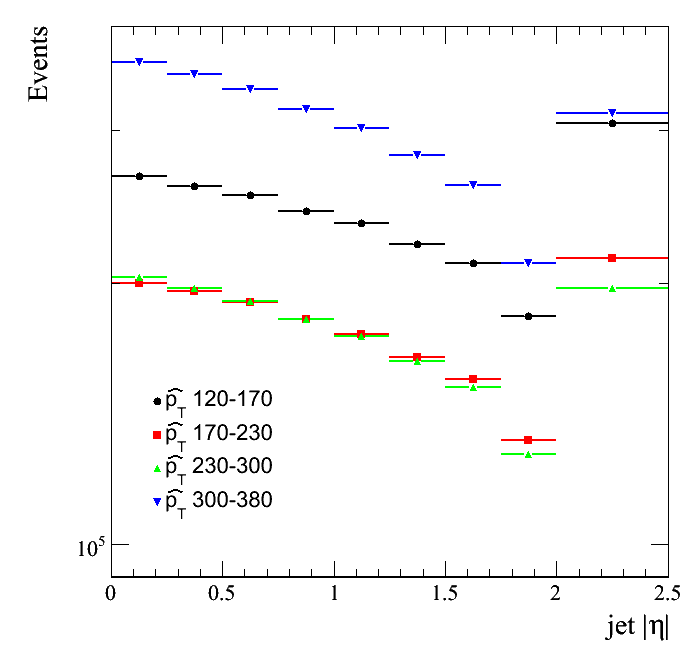
\includegraphics[width=80mm]{Figures/jet_eta_qcdbinned2.png}
  \end{center}
  \caption{Jet $p_T$ and $eta$ distributions from the QCD samples $120<\hat{p_T}<380$~GeV/c.}
  \label{fig:jet_pt_QCD2}
\end{figure}

\begin{figure}[htbp]
  \begin{center}
    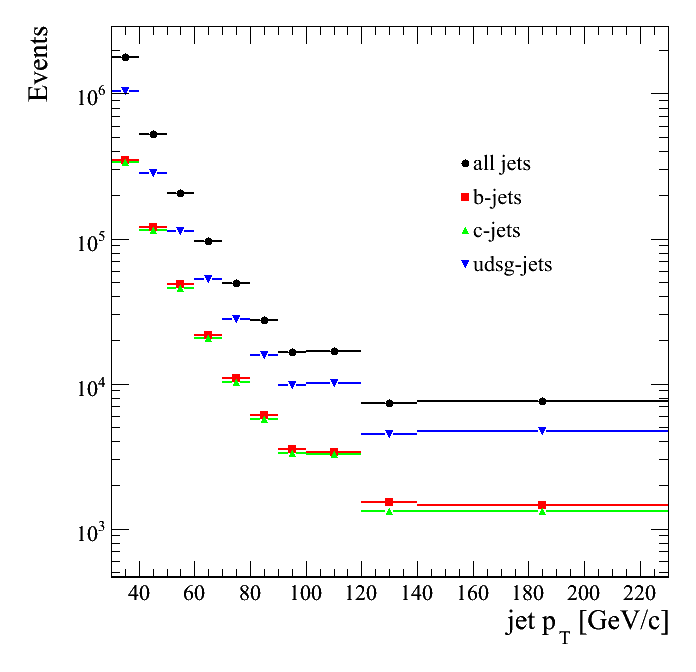
\includegraphics[width=80mm]{Figures/jet_pt_muX.png}
    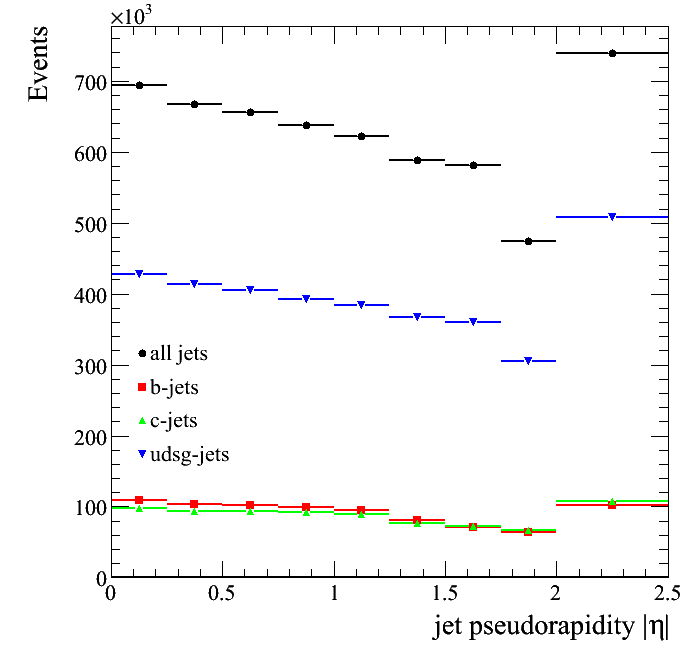
\includegraphics[width=80mm]{Figures/jet_eta_muX.png}
  \end{center}
  \caption{Jet $p_T$ and $eta$ distributions from the muon enriched QCD sample $pp\rightarrow \mu +X$}
  \label{fig:jet_pt_muX}
\end{figure}

\begin{figure}[htbp]
  \begin{center}
    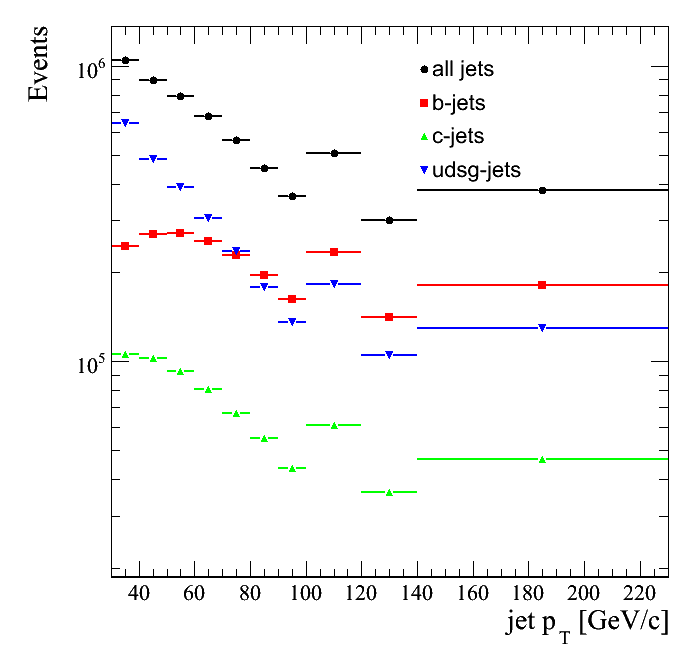
\includegraphics[width=80mm]{Figures/jet_pt_tt0j.png}
    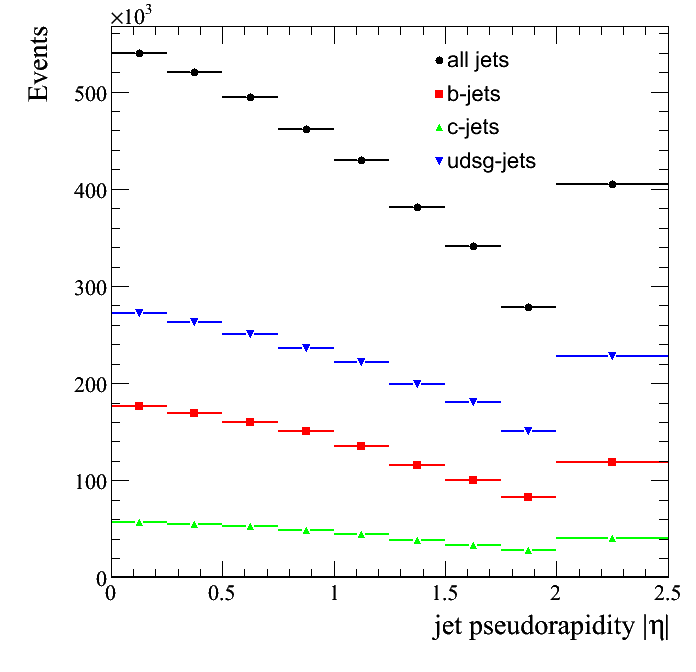
\includegraphics[width=80mm]{Figures/jet_eta_tt0j.png}
  \end{center}
  \caption{Jet $p_T$ and $eta$ distributions from the $t\bar{t}+0$~jets.}
  \label{fig:jet_pt_ttbar}
\end{figure}

\clearpage

\subsection{Muon $p_T$ with respect to muon+jet axis ($p_{Trel}$)}

\begin{figure}[htbp]
  \begin{center}
    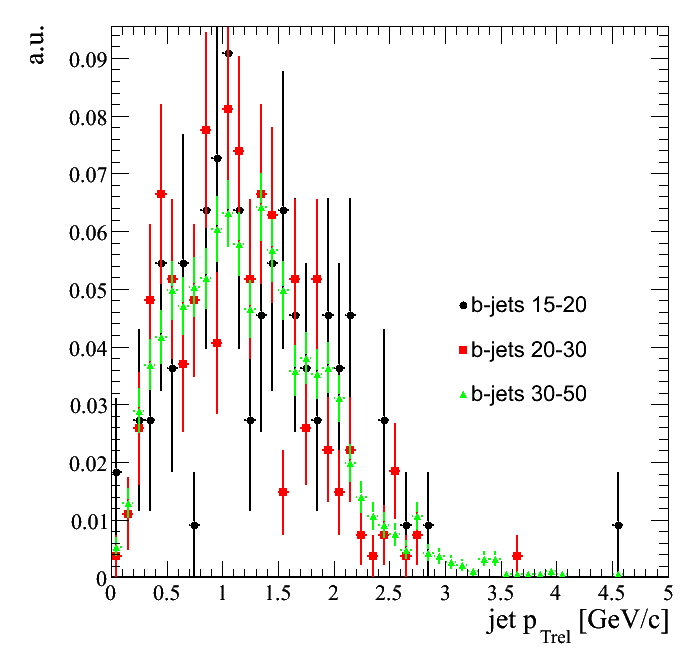
\includegraphics[width=80mm]{Figures/jet_ptrel_qcdbinned.png}
    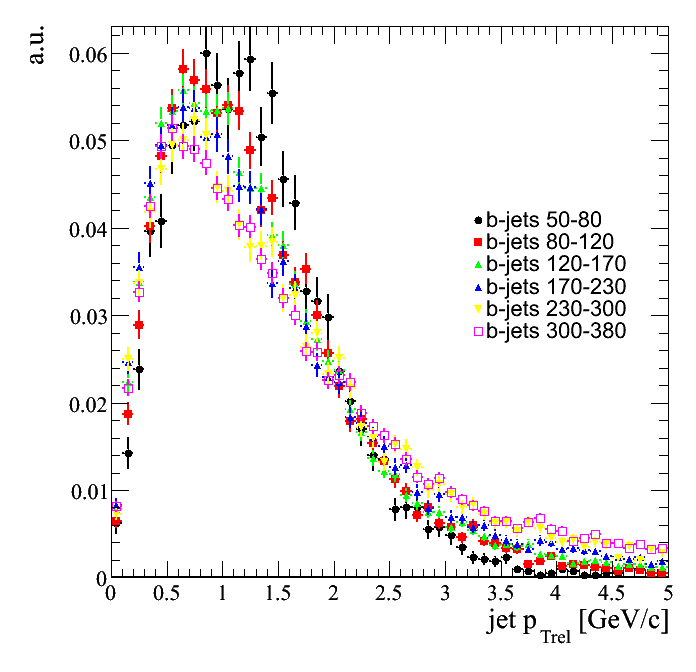
\includegraphics[width=80mm]{Figures/jet_ptrel2qcdbinned.png}
  \end{center}
  \caption{$p_{Trel}$ distribution from $b$ jets for low and high $\hat{p_T}$ bins from QCD sample.}
  \label{fig:jet_ptrel_b}
\end{figure}

\begin{figure}[htbp]
  \begin{center}
    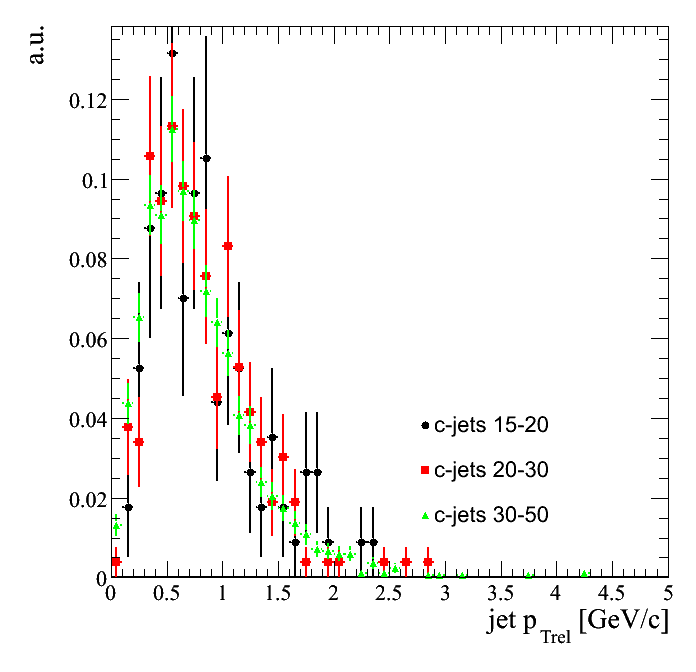
\includegraphics[width=80mm]{Figures/jet_ptrelcqcdbinned.png}
    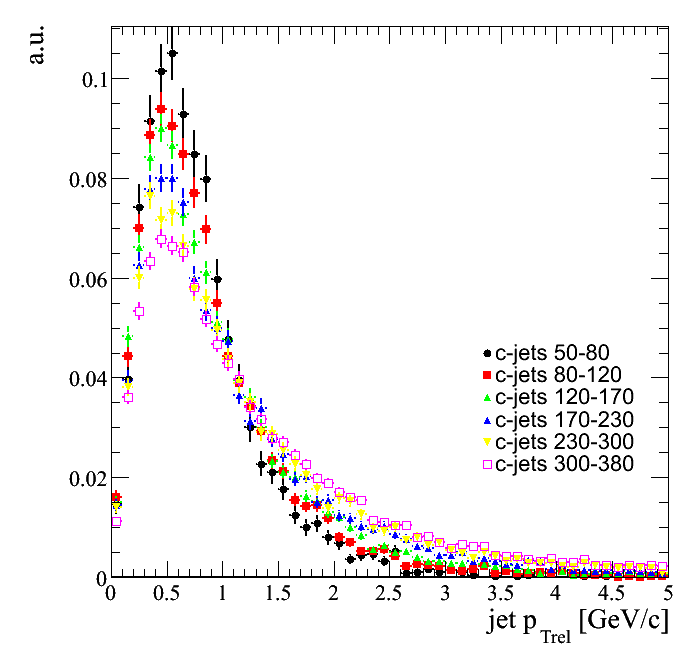
\includegraphics[width=80mm]{Figures/jet_ptrelcqcdbinned2.png}
  \end{center}
  \caption{$p_{Trel}$ distribution from $c$ jets for low and high $\hat{p_T}$ bins from QCD sample.}
  \label{fig:jet_ptrel_c}
\end{figure}


\begin{figure}[htbp]
  \begin{center}
    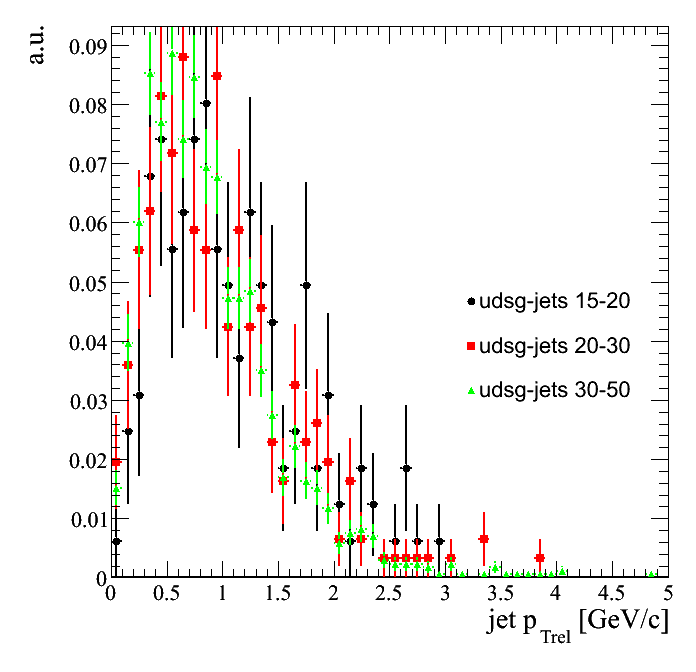
\includegraphics[width=80mm]{Figures/jet_ptreludsgqcdbinned.png}
    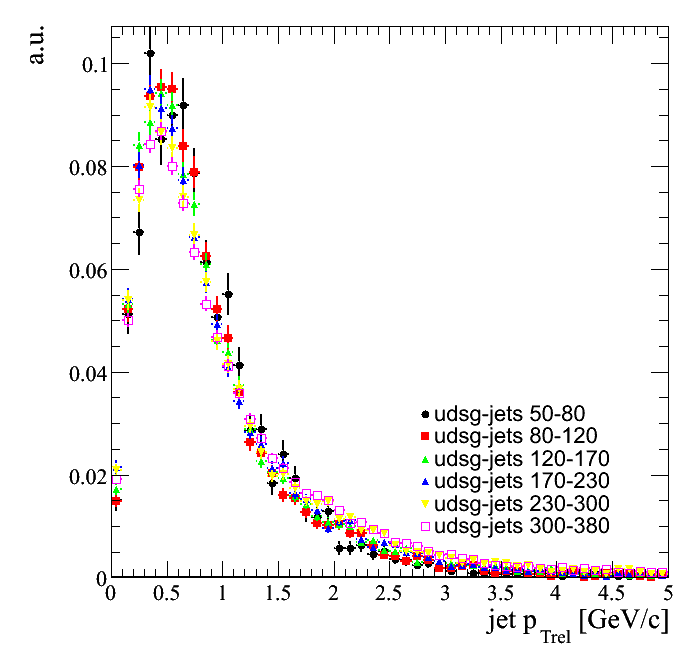
\includegraphics[width=80mm]{Figures/jet_ptreludsgqcdbinned2.png}
  \end{center}
  \caption{$p_{Trel}$ distribution from $udsg$ jets for low and high $\hat{p_T}$ bins from QCD sample.}
  \label{fig:jet_ptrel_udsg}
\end{figure}

\begin{figure}[htbp]
  \begin{center}
    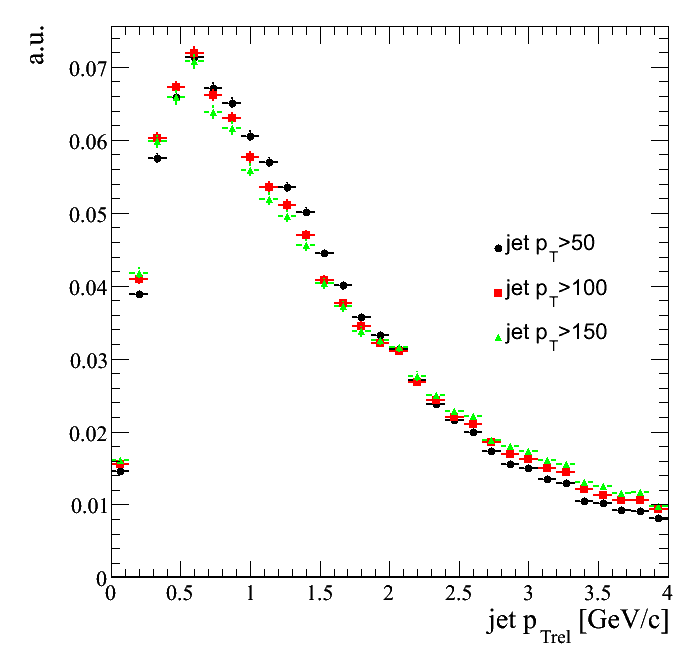
\includegraphics[width=80mm]{Figures/jet_ptrelb_jetcuts.png}
    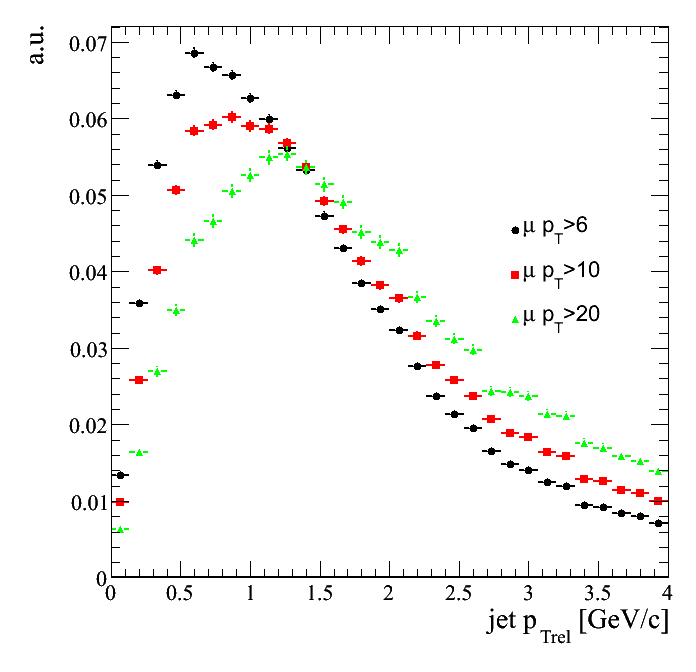
\includegraphics[width=80mm]{Figures/jet_ptrelb_mucuts.png}
  \end{center}
  \caption{$p_{Trel}$ distribution from $b$ jets with different jet $p_T$ (top) and muon $p_T$ (bottom) thresholds.}
  \label{fig:jet_ptrel_b_cuts}
\end{figure}

\begin{figure}[htbp]
  \begin{center}
    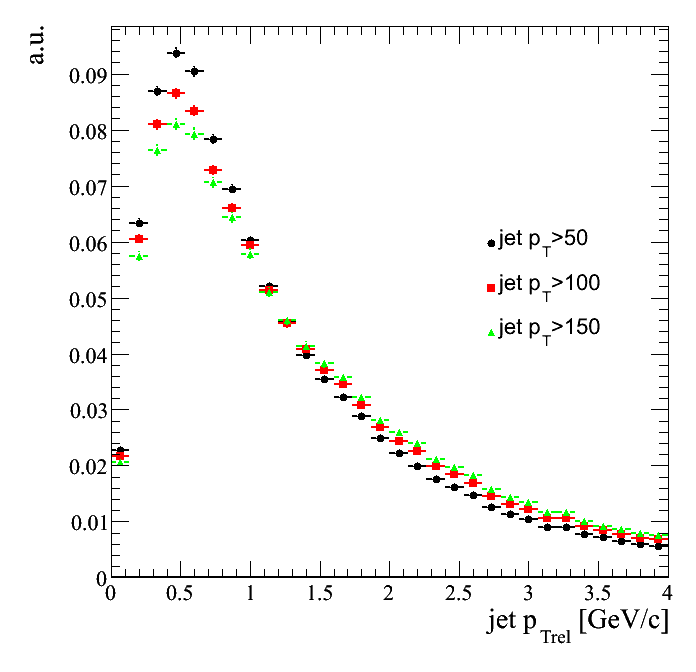
\includegraphics[width=80mm]{Figures/jet_ptrelc_jetcuts.png}
    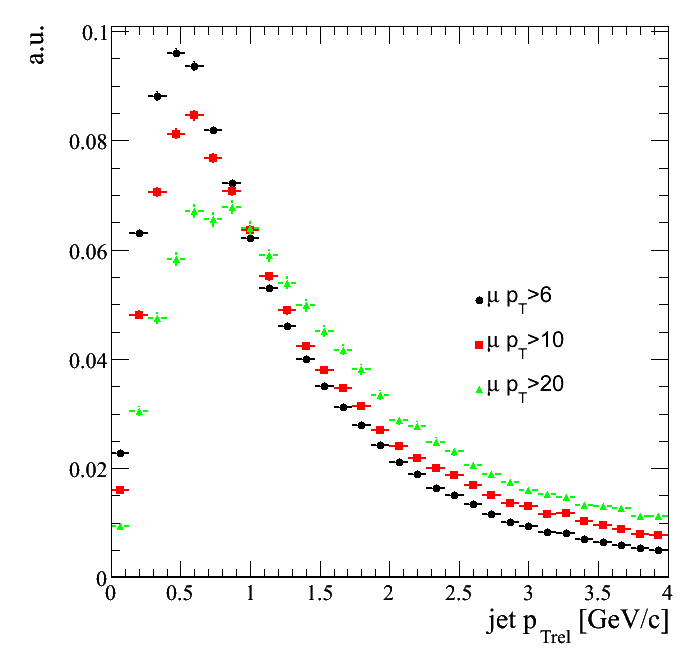
\includegraphics[width=80mm]{Figures/jet_ptrelc_mucuts.png}
  \end{center}
  \caption{$p_{Trel}$ distribution from $b$ jets with different jet $p_T$ (top) and muon $p_T$ (bottom) thresholds.}
  \label{fig:jet_ptrel_c_cuts}
\end{figure}

\begin{figure}[htbp]
  \begin{center}
    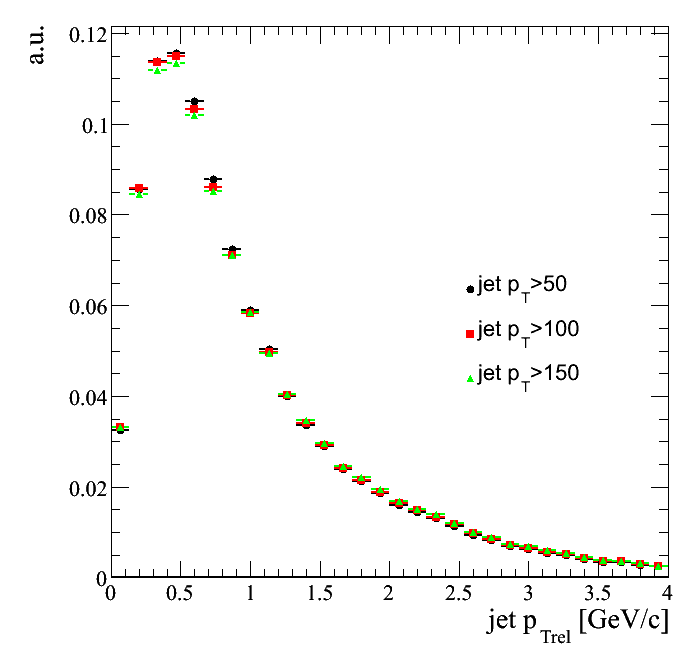
\includegraphics[width=80mm]{Figures/jet_ptreludsg_jetcuts.png}
    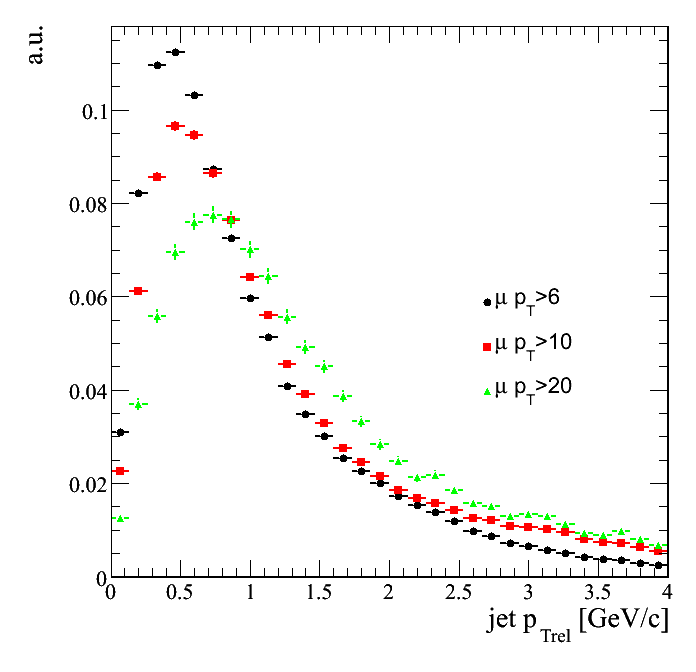
\includegraphics[width=80mm]{Figures/jet_ptreludsg_mucuts.png}
  \end{center}
  \caption{$p_{Trel}$ distribution from $udsg$ jets with different jet $p_T$ (top) and muon $p_T$ (bottom) thresholds.}
  \label{fig:jet_ptrel_udsg_cuts}
\end{figure}

\begin{figure}[htbp]
  \begin{center}
    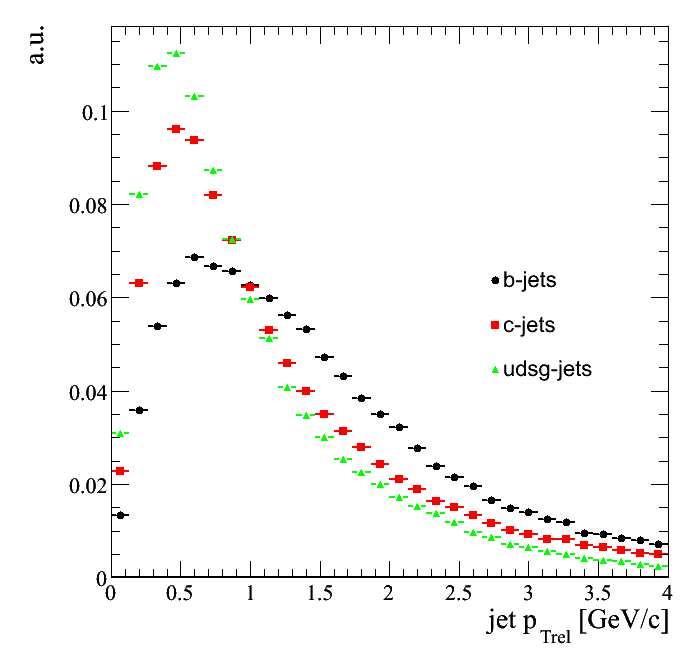
\includegraphics[width=80mm]{Figures/jet_ptrel_mu6.png}
    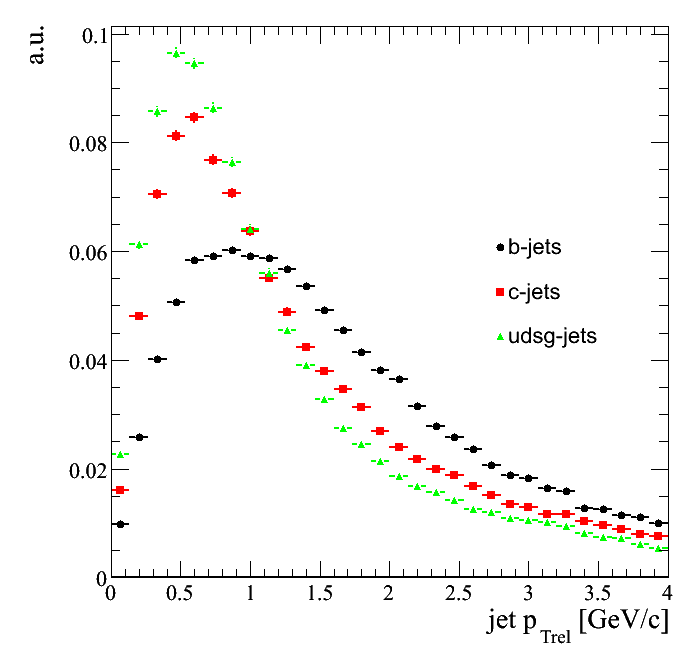
\includegraphics[width=80mm]{Figures/jet_ptrel_mu10.png}
    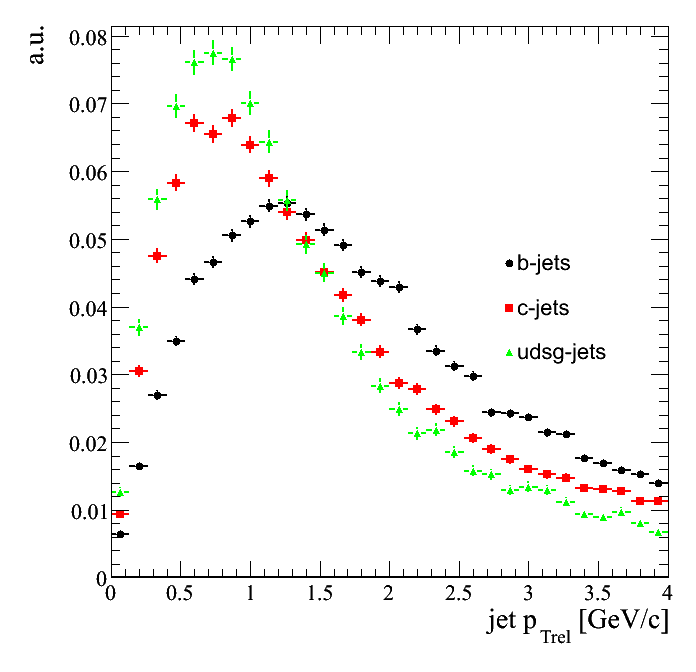
\includegraphics[width=80mm]{Figures/jet_ptrel_mu20.png}
  \end{center}
  \caption{$p_{Trel}$ distribution for $b$, $c$, and $udsg$ jets for muon $p_T>6$~GeV/c, $p_T>10$~GeV/c, $p_T>20$~GeV/c.}
  \label{fig:jet_ptrel}
\end{figure}

\begin{figure}[htbp]
  \begin{center}
    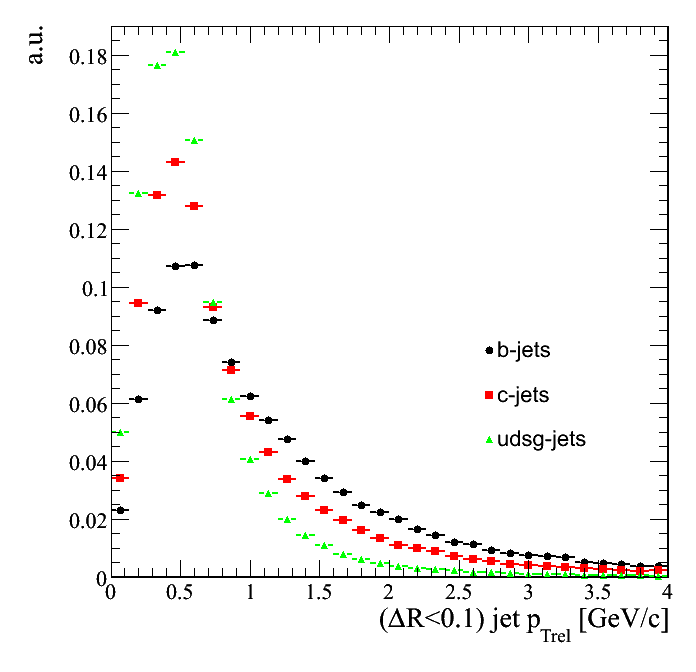
\includegraphics[width=80mm]{Figures/jet_ptrel_deltaR1.png}
    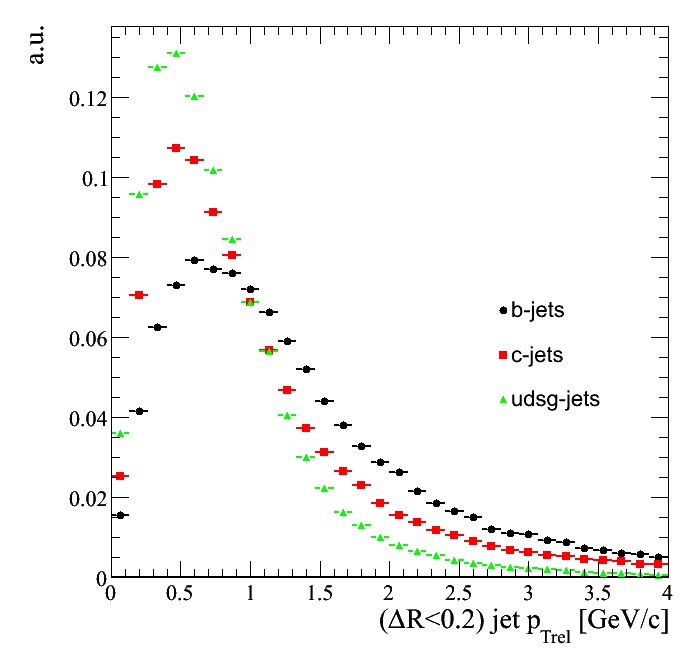
\includegraphics[width=80mm]{Figures/jet_ptrel_deltaR2.png}
    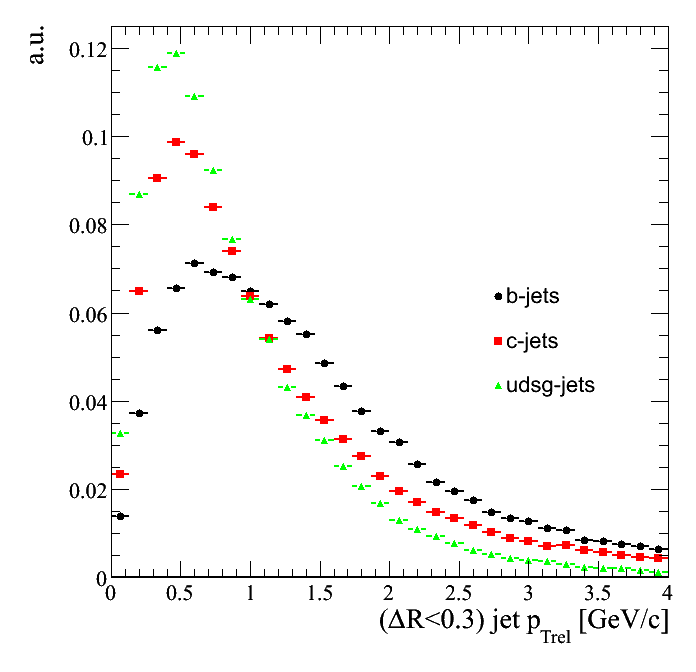
\includegraphics[width=80mm]{Figures/jet_ptrel_deltaR3.png}
  \end{center}
  \caption{$p_{Trel}$ distribution for $b$, $c$, and $udsg$ jets for $\Delta R(\mu,jet)<0.1$, $\Delta R(\mu,jet)<0.2$, and $\Delta R(\mu,jet)<0.3$.}
  \label{fig:jet_ptrel}
\end{figure}

\begin{figure}[htbp]
  \begin{center}
    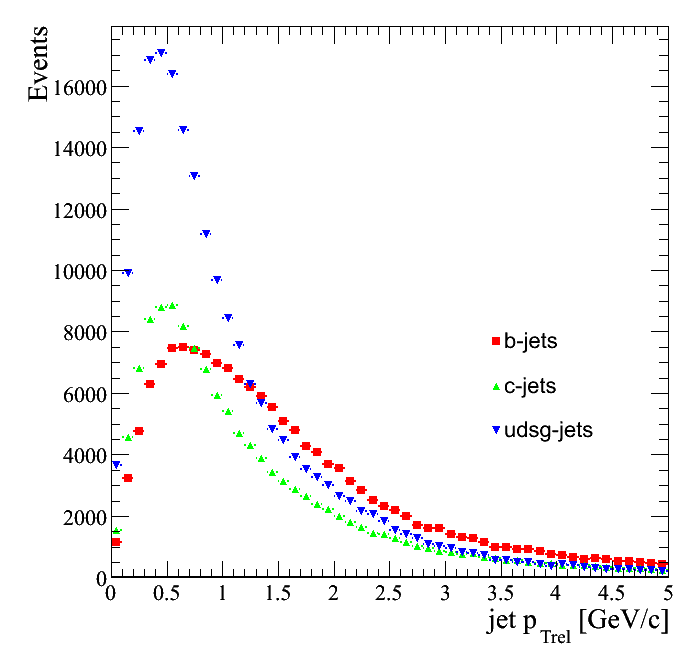
\includegraphics[width=80mm]{Figures/jet_ptrel_allqcd.png}
    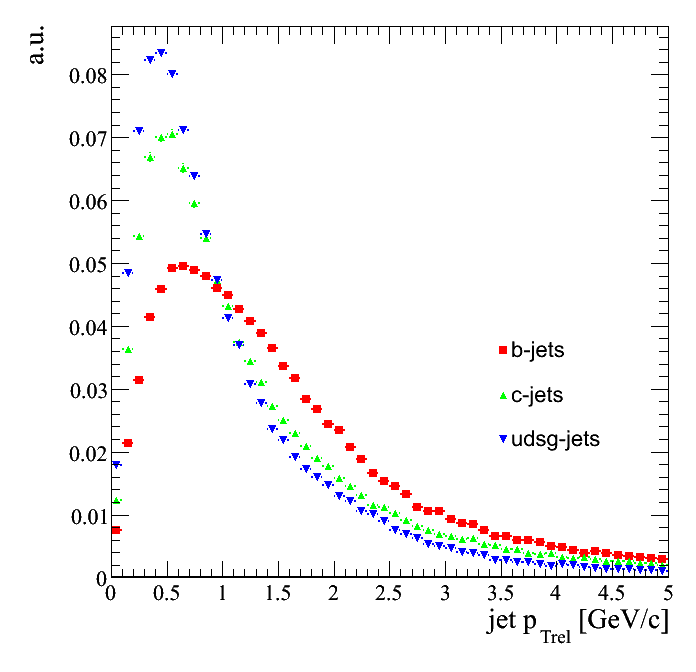
\includegraphics[width=80mm]{Figures/jet_ptrel_norm_allqcd.png}
  \end{center}
  \caption{$p_{Trel}$ distribution from the QCD sample. (bottom) Normalized distribution.}
  \label{fig:jet_ptrel_all_qcd}
\end{figure}


\begin{figure}[htbp]
  \begin{center}
    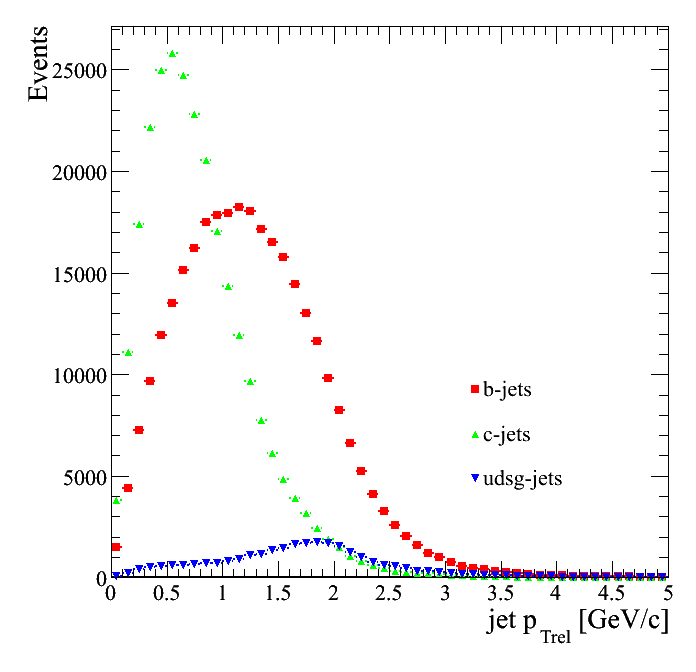
\includegraphics[width=80mm]{Figures/jet_ptrel_muX.png}
    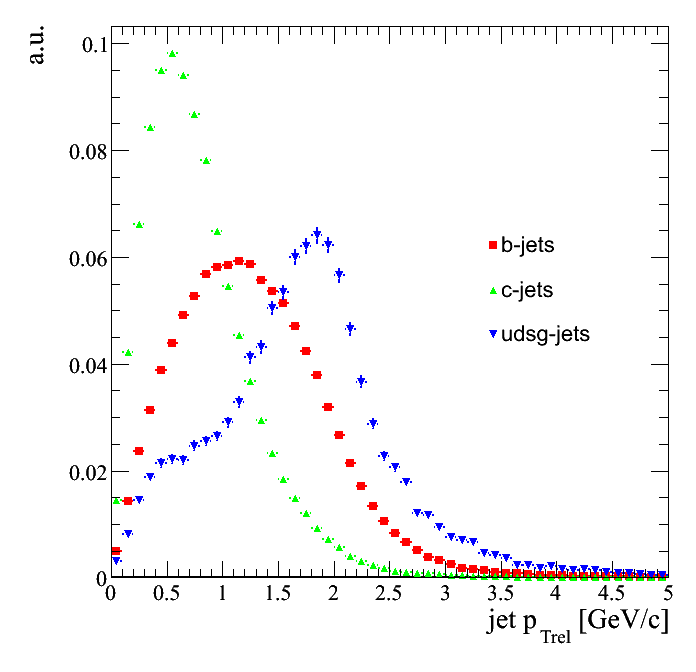
\includegraphics[width=80mm]{Figures/jet_ptrel_norm_muX.png}
  \end{center}
  \caption{$p_{Trel}$ distribution from the muon enriched QCD sample $pp \rightarrow \mu + X$. (bottom) Normalized distribution.}
  \label{fig:jet_ptrel_all_muX}
\end{figure}


\begin{figure}[htbp]
  \begin{center}
    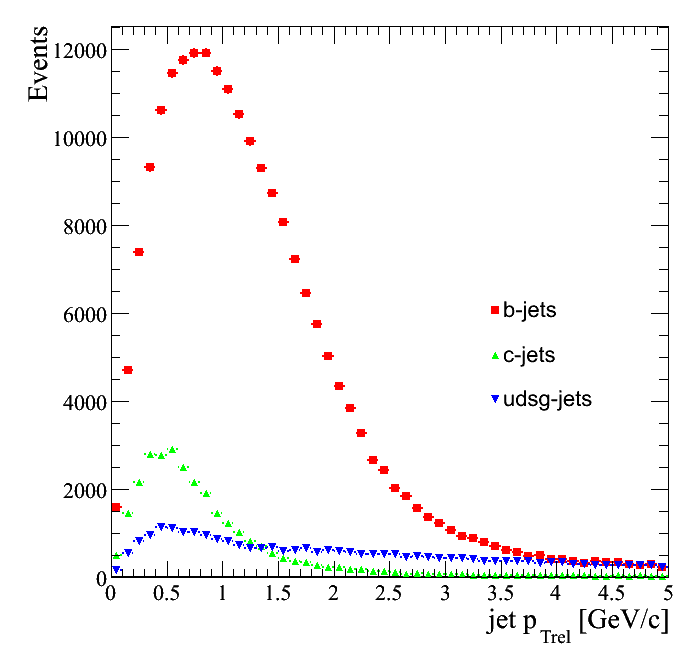
\includegraphics[width=80mm]{Figures/jet_ptrel_tt0j.png}
    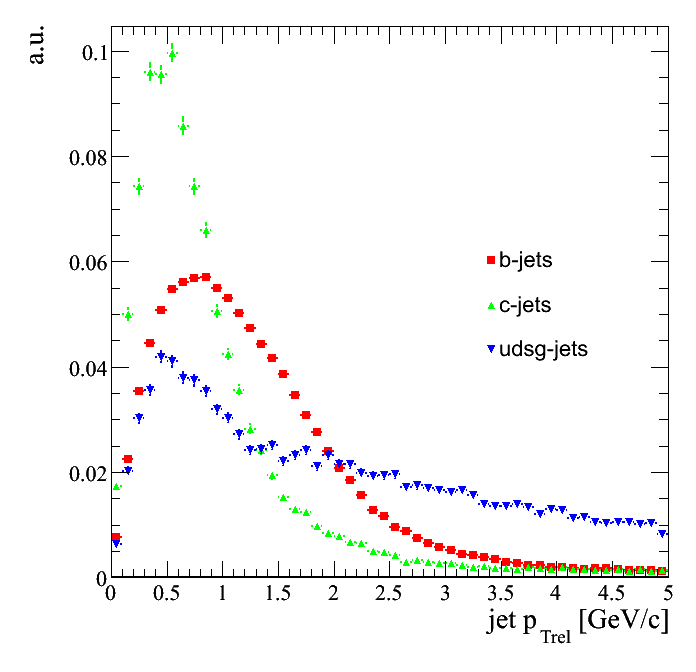
\includegraphics[width=80mm]{Figures/jet_ptrel_norm_tt0j.png}
  \end{center}
  \caption{$p_{Trel}$ distribution from the $t\bar{t}+0$~jets sample. (bottom) Normalized distribution.}
  \label{fig:jet_ptrel_all_ttbar}
\end{figure}


\clearpage

